%--------------------------------------------------------------------------
% Introduction
%--------------------------------------------------------------------------

\chapter{Introduction}
\label{cha: introduction}

\section{Background}
\label{sec: intro-background}

Forests are complex, functional systems of interacting and interdependent biological, physical, and chemical components, which creates unique combinations of climate, soil, plant and animal species that result in many different forest types around the world (\cite{blanco_forest_2012}). These ecosystems harbor the vast majority of biological species on Earth (\cite{pan_structure_2013}), account for 80\% of the Earth's total plant biomass (\cite{kindermann_global_2008}), and store more carbon in biomass and soils than is contained in the atmosphere. Forests not only play an important role in supporting and maintaining ecological systems and cycles, but also provide a broad range of goods and services to humanity, including social and economic benefits in the long term. Among the valuable ecosystem goods and services provided by forests are food, fibre, timber, medicine, clean water, aesthetic and spiritual values, climate regulation, a repository of carbon storage, and mitigation of natural hazards such as floods.


\section{Remote sensing of Philippine forests}
\label{sec: intro-rs-phil-forests}

In the Philippines, a nation-archipelago located between the equator and the Tropic of Cancer in Southeast Asia, forests harbor extremely high floral and faunal diversity, and at the same time also serve as home to upland communities that are highly dependent on forest resources. Studies have cited estimates of the extent of forest cover to be \url{~}90\% of the 30 M ha total land area of the Philippine islands before the Spanish colonisation in 1521, down to \url{~}70\% at the transition of colonial regimes between Spain and America by 1900s, and further reduced to \url{~}60\% during the Japanese occupation of the Philippines from 1942 to 1945. During the 20th century, the average deforestation rate in the Philippines was estimated to be 148,000 ha/yr. Recent official forestry statistics in 2015 reported a decline in forest cover from 7.17 M ha in 2003 to 6.84 M ha in 2010 (\cite{fmb_forestry_2015}). Timber harvesting and agricultural expansion during the Spanish colonisation, followed by rapid and extensive commercial logging in the 20th century were recognised as the main drivers of historical forest loss in the Philippines.

National forest surveys were conducted in the post-1950s period in support of managing the country's forest resources, which employed either ground-based forest surveys or spaceborne remote sensing technology to produce land and forest cover maps. To date, seven national forest surveys using remotely sensed data have been conducted in the Philippines (Table \ref{tab: intro-table1.1}).

\begin{spacing}{1.0}
\begin{longtable}[h!]{ p{1cm} p{5.4cm} p{2.2cm} p{1.9cm} p{2.5cm} }

    \caption[National forest surveys in the Philippines using remotely sensed data.]{National forest surveys in the Philippines using remotely sensed data.}
    \label{tab: intro-table1.1}\\
    
    	\toprule
    	Year & Source & Forest & Data & Method of\\ 
		{} & {} & Cover (\%) & Source & Interpretation\\ 
    	\midrule
    	\endhead
    	
		1973 & Lachowski et al. (1979) & 38.0 & Landsat & Digital\\
		1974 & Bruce (1977) & 29.8 & Landsat & Visual\\ 
		1976 & Bonita \& Revilla (1977) & 30.0 & Landsat & Visual\\ 
		1980 & Forestry Development Center (1985) & 25.9 & Landsat & Visual\\
		1987 & Swedish Space Corporation (1988) & 23.7 & SPOT & Visual\\
		2003 & National Mapping \& Resource Information Authority (2004) & No data & Landsat & Visual\\
		2010 & National Mapping \& Resource Information Authority (2014) & No data & Landsat, AVNIR & Visual\\ 
				
    	\bottomrule
    
\end{longtable}

	\noindent Note: At the time of its publication, Kummer's (1992b) study enumerated five national forest surveys using remotely sensed data conducted from the 1970s to the 1980s. Additional surveys conducted from 1990s to the present were included to update this list.\\ \newline
	
\end{spacing}

The forest cover maps generated from these past surveys were done mainly by the traditional method of visual or manual interpretation and analysis (except the 1973 maps) using optical remote sensing data, particularly Landsat. While visual interpretation of remotely sensed data is a simple and effective method that can result in excellent spatial information extraction, it is dependent on the extent of knowledge of the analyst regarding the area of study. Also, since the method depends solely on a human analyst it is more subjective, and tends to be tedious and slow compared to automated digital interpretation techniques.\\

\begin{spacing}{1.0}
\begin{longtable}[h!]{ p{7cm} p{7cm} }

    \caption[Forest cover classification systems used in the 1987, 2003, 2010 maps.]{Forest cover classification systems used in the 1987 and 2003/2010 forest maps.}
    \label{tab: intro-table1.2}\\
    
    	\toprule
    	1987 map & 2003/2010 map\\ 
    	\midrule
    	\endhead
    	
		Closed canopy, mature \textgreater 50\% & Closed forest, broadleaved\\
		Open canopy, mature \textless 50\% & Closed forest, coniferous\\
		Mossy forest & Closed forest, mixed\\
		Pine forest & Open forest, broadleaved\\
		Mangrove forest & Open forest, coniferous\\
		Marshy area and swamp & Open forest, mixed\\
		Submarginal forest & Forest plantation, broadleaved\\ 
		{} & Forest plantation, coniferous\\
		{} & Forest plantation, mangrove (2003 only)\\ 
		{} & Mangrove forest\\ 

    	\bottomrule \\
    
\end{longtable}	
\end{spacing}

The exclusive use of optical satellite data in these mapping surveys meant that cloud cover was a prevalent concern. In particular, tropical regions such as the Philippines feature persistent cloud cover, which affects data availability and temporal consistency of optical data, thereby preventing regular observations (\cite{myers_tropical_1988}). The lack of available optical data due to cloud cover contamination may be one of the major limiting factors in the application of the resulting map products from these forest surveys for periodic, consistent, and wall-to-wall national land and forest cover mapping and monitoring (Fig. \ref{fig: intro-fig1.1}).

Different forest classification systems were also adopted in these forest surveys. For example, the 2003 and 2010 NAMRIA maps employed similar forest classification schemes based on the FAO Global Forest Resources Assessment (GFRA), but these maps differed from the 1987 Swedish Space Corporation (SSC) map that adopted a different system (Table \ref{tab: intro-table1.2}). The forest definitions used to produce the 1987 map and the 2003/2010 maps were also different from each other. These inconsistencies restrict the direct comparison of these maps and render the results incompatible for historical forest cover change analysis.\\

\begin{figure}[!ht] \centering
	\captionsetup[subfigure]{width=2.0in} % <-- Use this to control text which is poorly spaced under a subfigure. 
	\begin{subfigure}[t]{0.32\textwidth}
		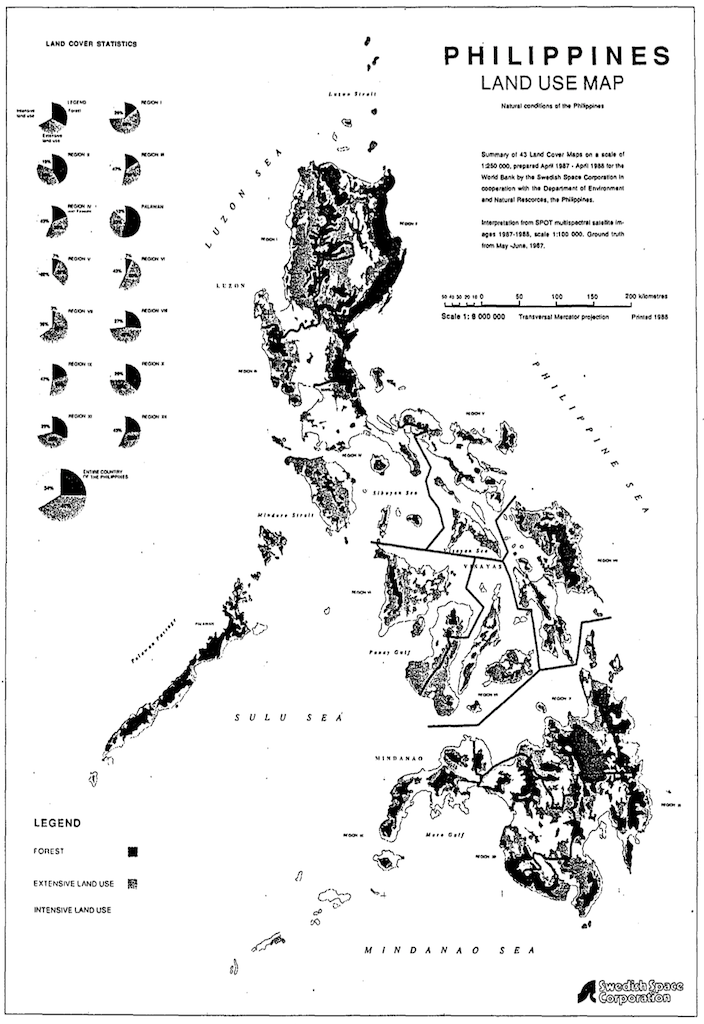
\includegraphics[width=\textwidth]{fig_1987-lc-map.png}
		\caption[SSC/NAMRIA land cover maps.]{}
		\label{fig: intro-fig1.1a}
	\end{subfigure}
	\begin{subfigure}[t]{0.32\textwidth}
		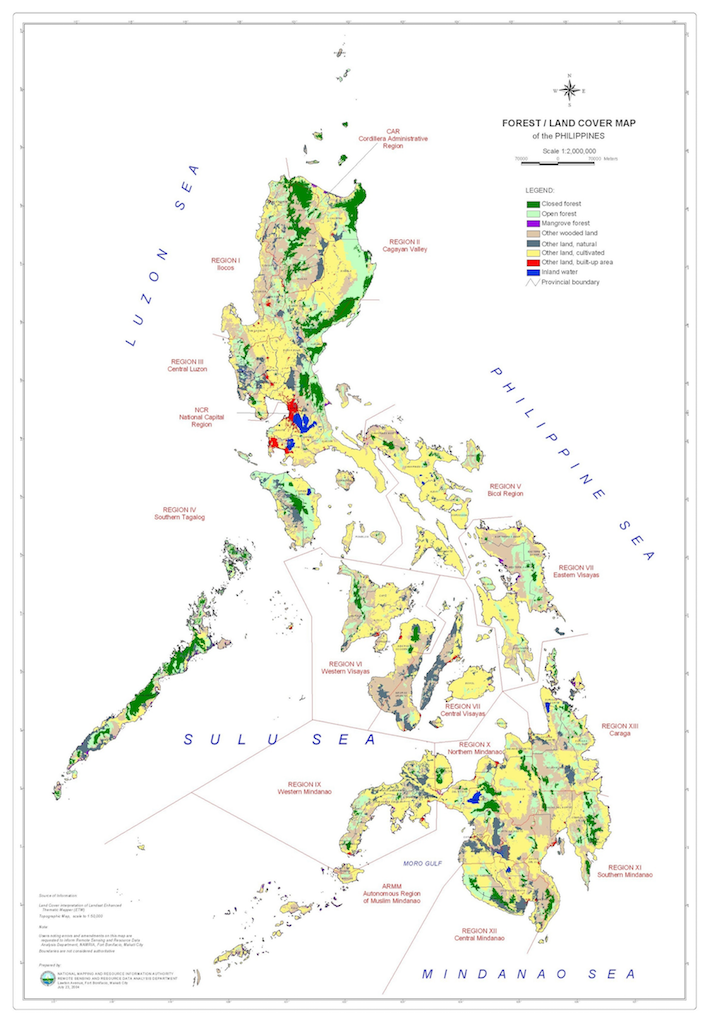
\includegraphics[width=\textwidth]{fig_2003-lc-map.png}
		\caption[SSC/NAMRIA land cover maps.]{}
		\label{fig: intro-fig1.1b}
	\end{subfigure}
	\begin{subfigure}[t]{0.32\textwidth}
		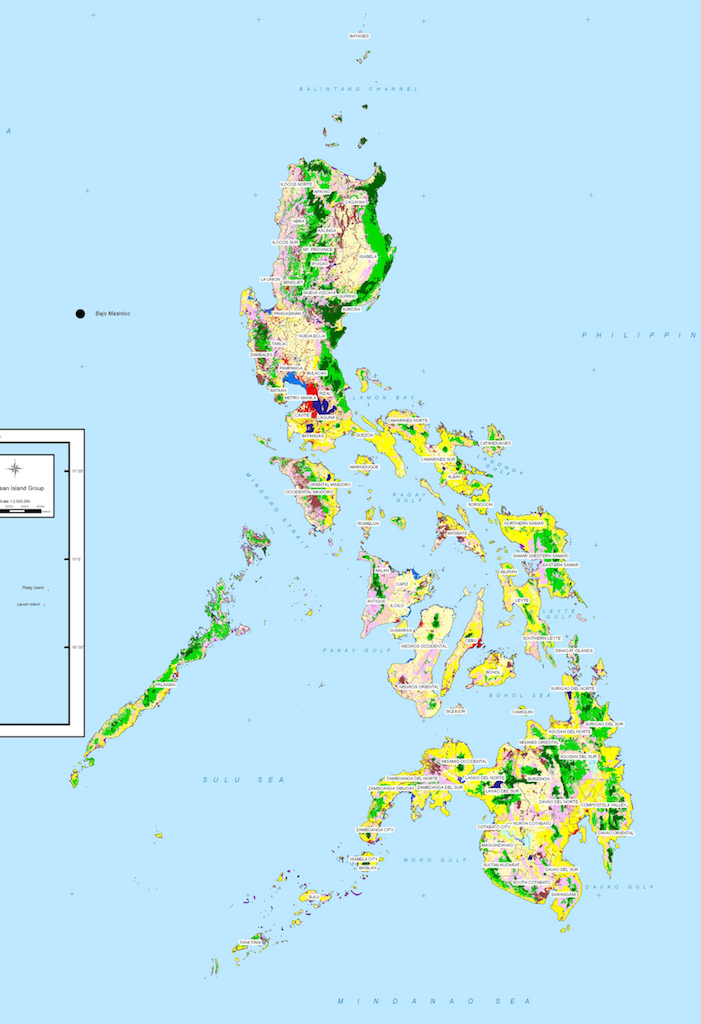
\includegraphics[width=\textwidth]{fig_2010-lc-map.png}
		\caption[SSC/NAMRIA land cover maps.]{}
		\label{fig: intro-fig1.1c}
	\end{subfigure}
	\caption[Recent national land cover maps of the Philippines: (a) 1987 SSC; (b) 2003 NAMRIA; (c) 2010 NAMRIA.]{Recent national land cover maps of the Philippines: (a) 1987 SSC; (b) 2003 NAMRIA; (c) 2010 NAMRIA.}
	\label{fig: intro-fig1.1}
\end{figure}

Finally, there is little known documentation that exists to report on the methods implemented and levels of accuracy achieved in producing many of the forest cover maps from these surveys, except the 1973 and 1987 maps. Lachowski et al. \citeyearpar{lachowski_landsat_1979}, for the 1973 Landsat-based maps, described the methods undertaken by the mapping work and mentioned an overall accuracy of 85\% to 95\% for the classification of forest types, albeit without sufficient detail. For the 1987 SPOT-based maps, SSC \cite{swedish_space_corporation_mapping_1988} described their methods and land cover classification system, but did not quantify the accuracy of the results of their interpretation. Kummer's study had cautioned on the reliability of the 1987 SSC map due to major differences with the results of the 1988 Philippine-German Forest Inventory (\cite{kummer_remote_1992}). Reports for other mapping surveys were either not (or no longer) available or were not easily accessible. Since many of these forest mapping surveys employed visual interpretation techniques implemented by expert analysts, the absence of documentation also affects the replicability of the approaches for future work since the knowledge developed from these surveys were ultimately lost.
